\section{Results}
\label{sec:Res}

% ----------------------------------------------------------------------- %
% ----------------------------------------------------------------------- %
\subsection{Classification Accuracies}
\label{sec:supp_tspec_res}

\subsubsection*{Effect of Support Size and Threshold}

Evaluating the uncalibrated tree species predictions revealed a dependency of the classification accuracies on both the applied threshold and the support size. Firstly, increasing the threshold led to a decrease in the user's accuracies for most of the tree species independent of the support choice (Fig. \ref{fig:cos_oaa_ua}). The reason for this is that raising the threshold to higher values leads to a higher probability for the reference class than for the predicted class to be assigned as class 'Mixed'. This is due to the distinct difference in the spatial resolution between the reference and prediction data: the rather coarse spatial resolution of the tree species raster map causes the predicted class to remain classified as one of the five tree species much longer than the reference data, which consist of individual sample trees of a sample location. This effect is amplified by high thresholds. The probability of the predicted class to also be classified as 'Mixed' can however be raised by increasing the number of raster cells to be evaluated. For this reason, the user's accuracies improve when using larger support sizes, and this effect is most pronounced under high thresholds. This scale-threshold dependency of the user's accuracy particularly affects tree species that most commonly occur in mixed forest stands in Rhineland-Palatinate, i.e. \textit{Scots pine}, $oak$ and $beech$. The user's accuracies for tree species that are mostly prominent in pure forest stands ($spruce$, \textit{Douglas fir}) logically turned out to be much more robust to changes in the thresholds and support sizes. Among the uncalibrated tree species predictions, $beech$ and $spruce$ produced the best predictions achieving UAs of up to 70\% and 80\%.  Although the predictions for \textit{Douglas fir} and \textit{Scots pine} generally performed less well than $beech$ and $spruce$, similar UAs can be produced by adjusting the threshold and support choices. UAs for $oak$ never performed better than 50\%. A detailed table of the user's and overall accuracies is provided in Online Resource 3.

%Evaluating the uncalibrated tree species predictions revealed a dependency of the classification accuracies on both the applied threshold and the support size. Firstly, increasing the threshold led to a decrease in the user's accuracies for most of the tree species independent of the support choice (Figure \ref{fig:cos_oaa_ua}). The reason for this is that raising the threshold to higher values leads to a higher probability for the reference class than for the predicted class to be assigned as class 'Mixed'. This is due to the distinct difference in the spatial resolution between the reference and prediction data: the set of individual sample trees of a sample location is much more prone to not exceed a high threshold than the evaluated pixels of the tree species raster map. As a result, the much coarser spatial resolution of the tree species raster map causes the predicted class to remain classified as one of the five tree species much longer than the reference data, particularly under high thresholds. The probability of the predicted class to also be classified as 'Mixed' can however be raised by increasing the number of raster cells to be evaluated by the threshold. For this reason, the user's accuracies improve when using larger support sizes, and this effect is most pronounced under high thresholds. This scale-threshold dependency of the user's accuracy particularly affects tree species that most commonly occur in mixed forest stands in Rhineland-Palatinate, i.e. \textit{Scots pine}, $oak$ and $beech$. The user's accuracies for tree species that are mostly prominent in pure forest stands ($spruce$, \textit{Douglas fir}) logically turned out to be much more robust to changes in the thresholds and support sizes.\par




% ---------------------- %

%\changed{The lowest user's accuracies ($UA$) for the uncalibrated tree species variable were mostly realized using high thresholds of 80\% and 100\% (figure \ref{fig:cos_oaa_ua}).} A plausible reason for this is that raising the threshold to higher values increases the probability of the reference class (based on the sample trees of the sample location) to be assigned as class 'Mixed', while the much coarser spatial resolution of the tree species map causes the predicted class to remain classified as one of the five tree species. 
%
%
%However, as the support size is  increased, so does the number of tree species raster cells to be evaluated at the sample location, thereby increasing the probability that the predicted class will also be 'Mixed'. For this reason, most tree species exhibit an increase in user's accuracy under higher thresholds with higher support sizes. This scale-threshold dependency of the user's accuracy particularly affects tree species that most commonly occur in mixed forest stands in Rhineland-Palatinate (\textit{Scots pine}, $oak$ and $beech$). The user's accuracies for tree species that are mostly prominent in pure forest stands ($spruce$, \textit{Douglas fir}) logically turned out to be much more robust to changes in the thresholds and support sizes.\par
%Among the uncalibrated tree species predictions, $beech$ and $spruce$ produced the best predictions achieving UAs of up to 70\% and 80\%.  Although the predictions for \textit{Douglas fir} and \textit{Scots pine} generally performed less well than $beech$ and $spruce$, similar UAs can be produced by adjusting the threshold and support choices. UAs for $oak$ never performed better than 50\%. A detailed table of the user's and overall accuracies is provided in Online Resource 3.

\begin{figure}
	\centering
	\resizebox{0.79\hsize}{!}{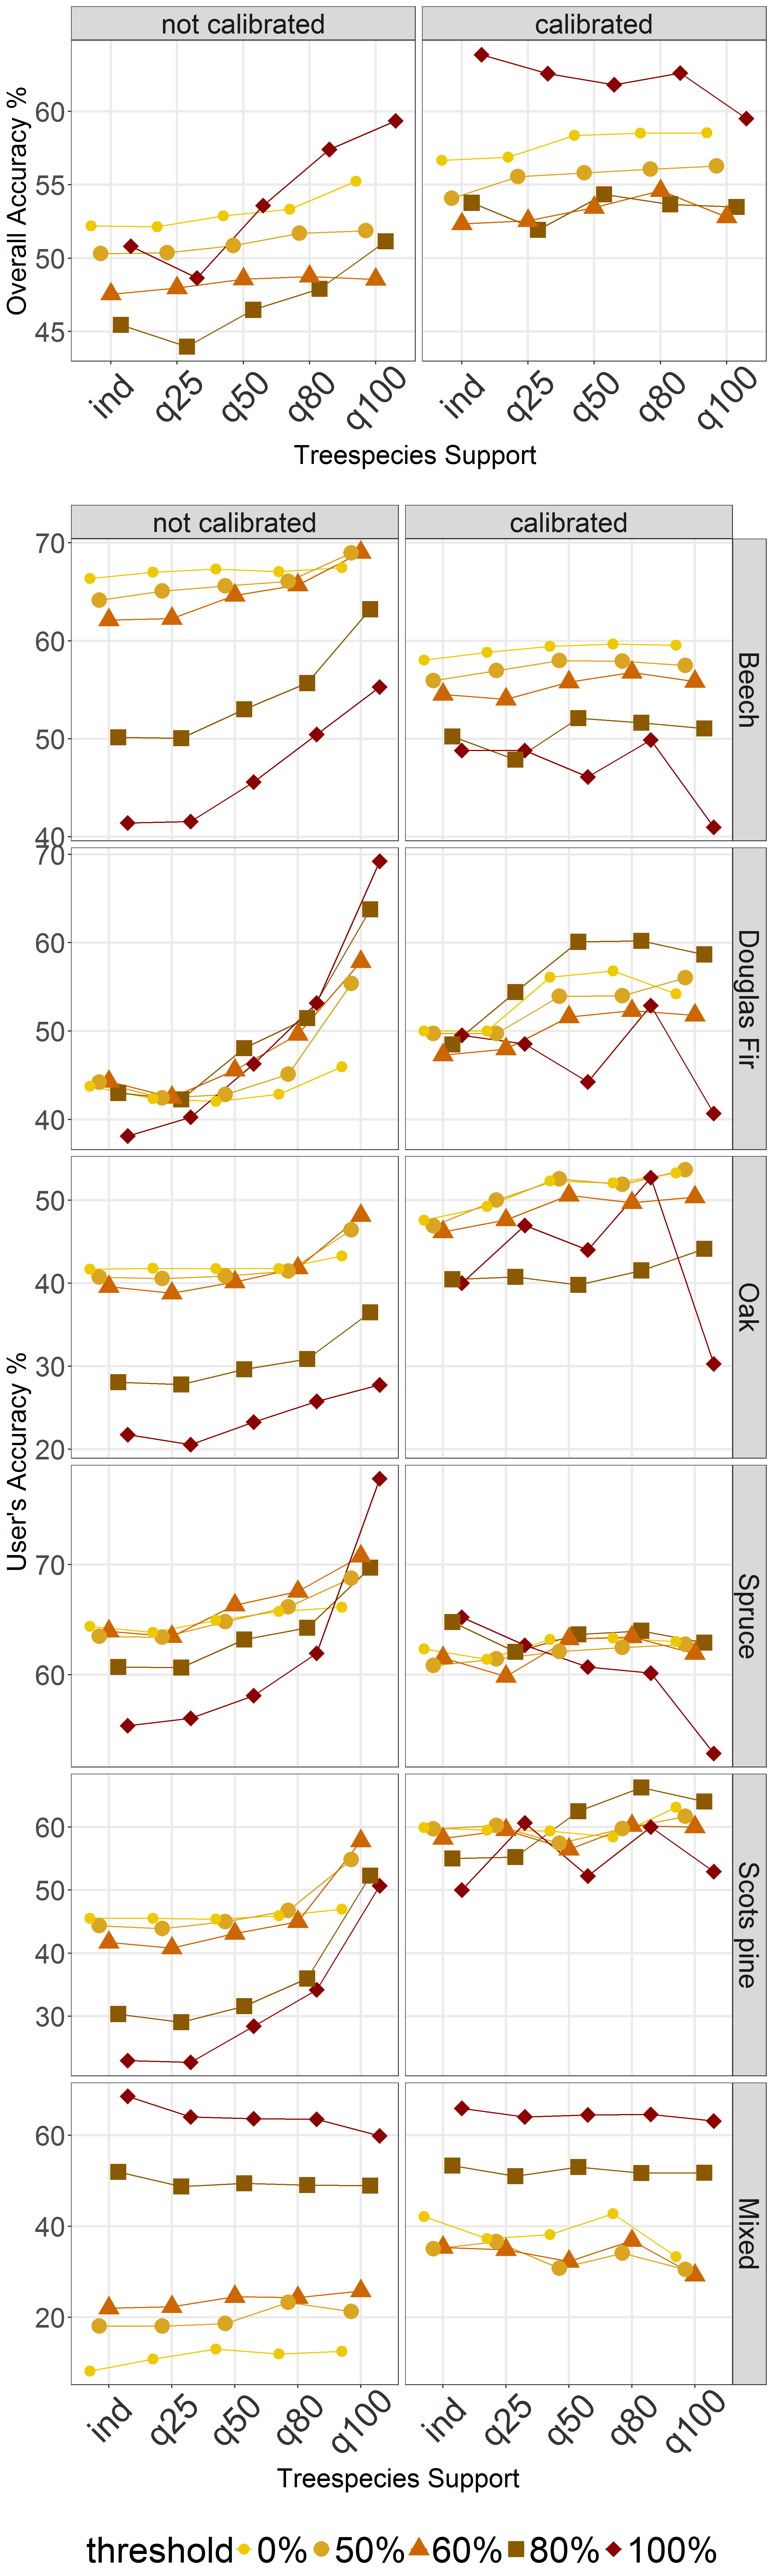
\includegraphics{oaa_and_cos_tspec_mixed_cal_nocal.png}}
    \caption{Classification accuracy for the main tree species of a sample location \textit{before} and \textit{after} calibration: \textit{top)} overall accuracies. \textit{bottom)} user's accuracies. \textit{ind}: plot individual support sizes.}
	\label{fig:cos_oaa_ua}
\end{figure}



\subsubsection*{\changed{Calibration}}
Calibration substantially diminished the effect of the scale-threshold dependency for the five tree species and also increased the UAs for \textit{Scots pine} and $oak$. \changed{Whereas the UAs for $beech$ and $spruce$ were found to be slightly lower after calibration,} the overall accuracy under each support choice was always considerably increased by calibrating the tree species prediction (Fig. \ref{fig:cos_oaa_ua}). With respect to the calculated random forest models, the initial tree species prediction ($treespecies$) and the information about the growing region ($wgb$) turned out to be the most valuable information, followed by the estimated proportion of coniferous trees ($prop.conif$) and the mean canopy height ($meanheight$).


% ----------------------------------------------------------------------- %
% ----------------------------------------------------------------------- %
\subsection{Regression Model Accuracies}
\label{sec:supp_chm_tspec_res}


\subsubsection*{Effect of Support Size and Threshold}

Figure \ref{fig:supp_perf_res} shows the accuracies of the regression model (Eq. \ref{eq:chmtspec_fullmod_term}) achieved under all possible combinations of support sizes for the auxiliary data. The stepwise selection procedure always included all considered single and interaction terms. In terms of \adjrsq{} and \rmsecv{}, the analysis revealed that the choice of the CHM support size controls the overall level of the model's accuracy. The information about the main plot tree species can then be used to further improve the model fit under suitable $treespecies$ support and threshold settings. When using the uncalibrated $treespecies$ variable, an increase of the $treespecies$ support size causes an increase in the model performance if low thresholds are used, whereas high thresholds (80\%, 100\%) cause a decrease in the model performance. This threshold-dependency could be removed by calibrating the $treespecies$ variable. \changed{The highest \adjrsq{} and the lowest \rmsecv{} were realized using the $q50$ support for both the CHM and calibrated $treespecies$ variables in combination with a $treespecies$ threshold of 100\%, resulting in (\adjrsq{} of 0.48 and \rmsecv{} of 136.62 m$^2$/ha (43.8\%).} However, various support and threshold combinations for the CHM and $treespecies$ variables can be used to yield almost identical \rmsecv{} and \adjrsq{} values. A detailed table of the model accuracies is given in Online Resource 4.

\begin{figure*}
\centering
\resizebox{0.8\hsize}{!}{\includegraphics*{cos_cal_nocal_bw.png}}
\caption{10-fold \rmsecv{}[\%] and \adjrsq{} realized under various support choices for the CHM and $tree species$ explanatory variables}
\label{fig:supp_perf_res}
\end{figure*}

\begin{figure*}
	\centering
	\resizebox{0.6\hsize}{!}{\includegraphics*{cos_r2_cal_vs_nocal.png}}
	\caption{Effect on the \adjrsq{} when substituting the actual main tree species with the predicted  main tree species of a sample plot. Each point in the graph represents the timber volume regression model under different supports and threshold settings. The \textit{dotted} line tracks the the model with the highest \adjrsq{} under the use of the error-free \textit{treespecies} variable. Semitransparent colours for the data points are used to visualize overlap.}
	\label{fig:supp_r2_calnocal}
\end{figure*}

\subsubsection*{Effect of Misclassifications}

\changed{We accessed the magnitude of the misclassification effect for all models that were analysed in Section \ref{sec:supp_chm_tspec_res}, i.e. for all possible support and threshold combinations for the CHM and $treespecies$ predictor variables. We first compared the \adjrsq{} of each model when using the uncalibrated $treespecies$ variable against the \adjrsq{} using the actual, i.e. error-free variable. We then did the same comparison for the model using the calibrated treespecies predictor variable. Figure \ref{fig:supp_r2_calnocal} provides a visualization of this comparison. Note that only the model with the predicted tree species variables can be applied to additional sample locations where no terrestrial survey has been carried out.}\\
As expected, the highest \adjrsq{} for every evaluated model was always achieved using the error-free tree species variable, whereas the missclassifications in the tree species variable led to a systematic decrease of the model accuracy. The calibration of the initially predicted main plot tree species using the random forest classification algorithm (Section \ref{sec:tspecclass}) turned out to not only improve the classification accuracies (Section \ref{sec:supp_tspec_res}), but also to considerably decrease the effect of the missclassifications on the regression model predictions and accuracy. Figure \ref{fig:supp_r2_calnocal} ($right$) shows that the \adjrsq{} under the actual and the calibrated predicted tree species variable are in general much closer to, and in many cases even on the identity line. \added{The differentiation into two distinct point clouds results from the poor model performance under support size $q100$ for the CHM variables (i.e. the lower point cloud).} Whereas the misclassifications in the uncalibrated $treespecies$ variable led to a residual inflation of \changed{0.01 - 0.05} in \adjrsq{}, it was only between \changed{0 and 0.01} after calibration. Further analysis revealed that when using the calibrated $treespecies$ variable, the regression coefficients were almost identical to the ones received using the actual main plot tree species.

%\begin{figure*}
%\centering
%\resizebox{0.63\hsize}{!}{\includegraphics*{cos_r2_cal_vs_nocal.png}}
%\caption{Effect on the \adjrsq{} when substituting the actual main tree species with the predicted  main tree species of a sample plot. Each point in the graph represents the timber volume regression model under different supports and threshold settings. The \textit{dotted} line tracks the the model with the highest \adjrsq{} under the use of the error-free \textit{treespecies} variable. Semitransparent colours for the data points are used to visualize overlap.}
%\label{fig:supp_r2_calnocal}
%\end{figure*}


% ----------------------------------------------------------------------- %
% ----------------------------------------------------------------------- %
\subsection{Final Regression Model}
\label{sec:regmod_final}

In order to address research questions 1 and 2 (i.e. the gain in model accuracy by tree species information and effect of heterogeneity in the ALS data), we investigated the model properties in more detail. For this purpose, we decided to use the best found model that was achieved under the support settings of $q50$ for both auxiliary data with a threshold of 100\% for the tree species variable as the regression model of choice. The reason for inspecting this model was that \textit{a)} the model provided the highest \adjrsq{} among all validated models while reducing the data handling complexity for upcoming applications (i.e. identical support sizes for all remote sensing data) and \textit{b)} the calibration neutralized the effects of misclassifications on the model predictions. The interaction term between $meanheight^2$ and $treespecies$ (i.e. considering separate curvatures for each tree species) turned out not to have a significant influence on the model accuracy and was dropped, resulting in an \adjrsq{} of 0.48 and a slightly increased \rmsecv{} of 140.62 m$^2$/ha (46.7\%). \added{The final model thus comprised 39 parameters (regression coefficients), i.e. the intercept, 3 main effects for continuous variables, 13 main effects for categorical variables and 22 interaction parameters (Table \ref{tab:modacc_modterms}).\par
We also conducted an analysis for detecting influential data points or outliers for the final regression model. We here considered the commonly applied criteria of leverages and Cook's Distance as amongst others described in \citet[p. 160-167]{fahrmeir2013}. The critical threshold of $2p/n$ (i.e. twice the average of the hat matrix' diagonal entries) was exceeded by 10\% of the observations. However, only 3\% of these leverage points were assigned to studentized residuals with values $>$ 1 or $<$ -1. Removing these observations from the dataset and refitting the model led to an \adjrsq{} of 0.49 compared to 0.48 when including them. Additionally, Cook's Distance values $D_i$ did not exceed a value of 0.019, and were thus far apart from the commonly used critical threshold of $D_i >$ 0.5 that indicate a considerably change of the regression model results when omitting them. We thus decided not to remove any observations from the modelling dataset. We thus decided not to remove any observations from the modelling dataset.}


\subsubsection*{Interpretation of Final Regression Model}
\label{sec:prop_regmod_final}
Figure \ref{fig:predlines_tspec} provides a visualisation of the timber volume predictions separated by the calibrated tree species and the ALS acquisition years. Sample plots classified as $oak$ and \textit{Scots pine} revealed to have an almost identical relationship (nearly identical slopes) for the mean canopy height - timber volume relationship. They only differ by a marginally higher intercept for \textit{Scots pine} plots, meaning that given the same mean canopy height a sample plot dominated by \textit{Scots pine} yields a marginally higher timber volume on the plot level than a plot dominated by $oak$. $Beech$-dominated sample plots tend to achieve a higher timber volume than $oak$ and \textit{Scots pine} for canopy heights below 20 meters, but realize the lowest timber volumes for canopy heights above 20 metres. Sample plots dominated by any of the remaining coniferous tree species (\textit{Douglas fir}, $spruce$) revealed to have higher slopes than broadleaf classified plots. This indicates that given the same mean canopy height, sample plots dominated by \textit{Douglas fir} and $spruce$ yield higher timber volume values than broadleaf- or \textit{Scots pine} dominated sample plots, and this difference becomes more pronounced with increasing mean canopy heights. Within the group of coniferous-dominated sample plots, $spruce$ turned out to have the highest slope, thereby yielding the highest timber volume values for mean canopy heights above 15 meters. An undesired characteristic of the model is that the predicted timber volume can in some cases ($<$ 1\%) take negative values for low canopy heights (e.g. for $spruce$-dominated plots with \textit{meanheight} below 5 meters and $stddev$ of 4 meters). \changed{However, we chose not to use a log-transformation of the response variable. Doing so would have prevented the subsequent calculation of the g-weight variance of the design-based estimators \citep{mandallaz2013a, mandallaz2013b}, which is only possible for response variables on the original scale. The g-weight variance provides the benefit of a better variance estimate for internal models by considering the dependency of the regression coefficients on the realized sample. The rare occurrence of negative predictions were however not considered to have an influence on subsequent design-based estimates when averaging multiple predictions within given spatial domains.}

\subsubsection*{Effect of Time-Lags and Heterogeneity in ALS Data}

Incorporating the ALS acquisition year as a categorical variable ($ALSyear$) in the regression model substantially accounted for the variability in the data introduced by \textit{a)} the time-lags between ALS acquisition and terrestrial survey, and \textit{b)} variation in ALS data quality which are due to sensor- and post processing techniques (Table \ref{tab:modacc_modterms}). \changed{Whereas the \adjrsq{} for the regression model without considering the ALS acquisition year as additional predictor variable (\textit{submodel 1}) was 0.36, it could already been increased to 0.40 by including the tree species variable (\textit{submodel 2}). A further stratification by the ALS acquisition year increased the \adjrsq{} of \textit{submodel 1} from 0.36 to 0.45, and the \adjrsq{} of \textit{submodel 3} from 0.40 to 0.48.} 

% latex table generated in R 3.4.2 by xtable 1.8-2 package
% Sun Jan 07 17:26:28 2018
\begin{table}[ht]
	\centering
	\caption{$R^2$, RMSE and RMSE\% of final regression model within ALS acquisition year strata (\textit{ALSyear}). $Area_{ALSyear}$: Area covered by ALS acquisition given in km$^2$. \textit{n}: number of validation data.}
	\label{tab:adj_r2_within}
	\begin{tabular}{lllrrr}
		\hline
		\textit{ALSyear} & $Area_{ALSyear}$ & $R^2$ & RMSE & RMSE\% & n \\ 
		\hline
 2012 & 2807   & 0.61 & 135.84 & 44.87 & 408 \\ 
 2011 & 4361  & 0.57 & 146.21 & 48.29 & 883 \\ 
 2010 & 4182 & 0.51 & 120.90 & 39.93 & 1171 \\ 
 2009 & 2100 & 0.42 & 133.42 & 44.07 & 559 \\ 
 2008 & 2968 & 0.48 & 130.38 & 43.06 & 701 \\ 
 2008\_1 & 2116 & 0.33 & 175.43 & 57.94 & 394 \\ 
 2007 & 3498 & 0.46 & 136.47 & 45.08 & 418 \\ 
 2003 & 602 & 0.27 & 154.48 & 51.02 & 529 \\ 
 2002 & 775 & 0.44 & 141.55 & 46.75 & 314 \\ 
		\hline
\hline
\end{tabular}
\end{table}
%\end{longtable}
%\endgroup

%% old version
%\begin{table}[ht]
%	\centering
%	\caption{$R^2$, RMSE and Residual Square Sum (SSE) of final regression model within LiDAR acquisition year strata (\textit{lidaryear}). \textit{n}: number of validation data}
%	\label{tab:adj_r2_within}
%	\begin{tabular}{llrrr}
%		\hline
%		LiDAR acquisition year & $R^2$ & rmse & SSE & n \\ 
%		\hline
%		2012   & 0.55 & 139.54 & 7535278 & 387 \\ 
%		2011   & 0.55 & 145.21 & 17880553 & 848 \\ 
%		2010   & 0.48 & 122.16 & 16907662 & 1133 \\ 
%		2009   & 0.43 & 127.17 & 8652419 & 535 \\ 
%		2008\_1 & 0.34 & 170.49 & 11161424 & 384 \\ 
%		2008   & 0.50 & 124.39 & 10475374 & 677 \\ 
%		2007   & 0.49 & 129.72 & 6950192 & 413 \\ 
%		2003   & 0.32 & 146.37 & 11139814 & 520 \\ 
%		2002   & 0.43 & 139.79 & 6038601 & 309 \\ 
%		\hline
%		\hline
%	\end{tabular}
%\end{table}
%%\end{longtable}
%%\endgroup


We further analysed the model residuals within each ALS acquisition year (within-group variation) for the final model and nested submodels. It turned out that the $R^2$ values vary distinctly between the ALS acquisition year strata (Table \ref{tab:adj_r2_within}). More precisely, the within-group $R^2$ can be higher and lower than the overall $R^2$ of the respective model. Figure \ref{fig:r2adj_in_lyears} shows that a stratification according to the ALS acquisition years (submodel 2) can already increase the $R^2$ in most acquisition year strata, compared to the basic model using only the ALS height metrics as predictor variables (submodel 1). In the ALS acquisition year stratum 2007, the increase in $R^2$ even reached 0.08.

\begin{figure*}[h]
	\centering
	\resizebox{0.88\hsize}{!}{\includegraphics*{predlines_tspecaux_cal.png}}
	\caption{Visualization of the timber volume prediction function (\textit{final regression model}) on sample plot level for each main plot tree species and ALS acquisition year. For visualization purposes, the predictor variable $stddev$ was set to its average value within the respective \textit{treespecies} and \textit{ALSyear} categories. The terrestrially observed timber volume values are plotted in the background. \vspace{5mm}}
	\label{fig:predlines_tspec}
\end{figure*}


% \begingroup\fontsize{10pt}{11pt}\selectfont
\begin{table*}
\centering
\caption{Accuracy metrics for submodels of final OLS regression model} 
\label{tab:modacc_modterms}
\begin{tabular}{llrrr}
  \hline
model terms & model & parameters & $R^2_{adj}$ & \rmsecv{} \\ 
  \hline
meanheight + stddev + meanheight$^2$ + \\ treespecies + lidaryear + meanheight:treespecies + \\ meanheight:lidaryear + meanheight:stddev + \\ stddev:lidaryear & final model &  39 & 0.48 & 137.49 \\ \\
  meanheight + stddev + meanheight$^2$ + \\ meanheight:stddev & submodel 1 &   5 & 0.35 & 153.02 \\ \\
  meanheight + stddev + meanheight$^2$ + \\ lidaryear + meanheight:lidaryear + \\ meanheight:stddev + stddev:lidaryear & submodel 2 &  29 & 0.44 & 142.82 \\ \\
  meanheight + stddev + meanheight$^2$ + \\ treespecies + meanheight:treespecies + \\ meanheight:stddev & submodel 3 &  15 & 0.40 & 142.82 \\ 
   \hline
\hline
\end{tabular}
\end{table*}
%\endgroup





\subsubsection*{Added Value of Tree Species Map Information}
\changed{Introducing the predicted main tree species of a sample plot as an additional categorical variable to submodel 2 yielded a further increase in the \adjrsq{} of 0.03 (Table \ref{tab:modacc_modterms}). However, the improvement was even more pronounced in ALS acquisition years close or identical to the year of the terrestrial inventory (Fig. \ref{fig:r2adj_in_lyears}). We observed an increase of 0.06 in $R^2$ for ALS acquisition year 2012, and of 0.07 for ALS acquisition year 2011.} The analysis illustrated once more that misclassifications in the tree species variable generally reduce model accuracy compared to using error-free tree species information. The residual inflations caused by the misclassifications in the uncalibrated $treespecies$ variable within the $ALSyear$ strata were up to 0.05 in R$^2$. However, the calibration was able to substantially decrease or even remove the effects of misclassifications on the model accuracy in all ALS acquisition year strata.

\begin{figure}[H]
	\centering
	\resizebox{1\hsize}{!}{\includegraphics*{r2adj_in_lyears.png}}
	\caption{$R^2$-values of the final regression model, submodel 1 and submodel 2 achieved $within$ the ALS acquisition year strata.}
	\label{fig:r2adj_in_lyears}
\end{figure}

